\Chapter{Felhasznált technológiák és fejlesztői környezetek}

\Section{Backend}

A backend a web alkalmazás szerver oldala, amit nem lát a felhasználó. Itt szokott történni az adatbázissal való kommunikáció,továbbá az authentikáció(hitelesítés) és az authorizáció(engedélyezés). Nagyon sok féle backend technológia létezik mint, például: PHP, Python, Node.js és Java programozási nyelvek. A Javat fogom használni a fejlesztések során.

\subsection{Java}

A Java egy objektum orientált programozási nyelv, amit James Gosling fejlesztett a 90’-es években Sun Microsystemsnél. Eredetileg televíziózásra készült, de azokban az időkben túlságosan fejlett volt hozzá.

A java célja a hordozhatóság, ami azt jelenti, hogy a Java-ban írt programoknak hasonlóan kell futnia bármely JRE-vel rendelkező operációs rendszeren. Java nyelvi kódot először bájtkódra fordítják, ami hasonló a gépi kódhoz, de virtuális gép általi végrehajtásra készülnek. Vannak mikro vezérlők amik képesek a Java bájtkódját közvetlenül hardveren futtatni.

Java a szintaxisát a C és C++ nyelvből örökölte, még a C++ egyesíti a strukturált, általános és objektumorientált programozás szintaxisát addig a Java csak Objektumorientált nyelvnek készült. Java nem támogatja az operátok túlterhelést vagy a többszörös öröklődést (interfészek esetében lehetséges).

A java jelenlegi tulajdonosa az Oracle Corporation 2010-óta, miután felvásárolta a Sun Microsystems-t.

Java az egyik legelterjedtebb programozási nyelv, mivel az elterjedt operációs rendszerekre tudunk vele alkalmazást fejleszteni, és könnyen tanulható. Nagyon felhasználó barát\cite{Java}.

\subsection{Spring Boot}

A Spring Boot Spring-keretrendszerre épülő bővítmény a Spring pedig egy Java alapú webalkalmazás-keretrendszer, ami nyílt forráskódú. A Spring testreszabott webalkalmazások létrehozásához tökéletes, ami teljesen konfigurálható az előre elkészített kódterekkel és kódtárakkal. Spring Boottal különálló Spring alkalmazásokat hozhatunk létre, amit azonnal futtathatunk.

A Spring Boot használata nagyon egyszerű, jó minőségű alkalmazásokat lehet benne fejleszteni kevesebb fejlesztési idő alatt. Beépített HTTP-kiszolgálókat tartalmaz, mint a Tomcat és a Jerry.

A spring Boot tartalmaz egy Maven-hez tartozó (pom.xml) fájlt, amiben spring-boot-dependencies-eket tudunk megadni, mint például:

\begin{itemize}
\item spring-boot-starter-web,
\item spring-boot-starter-data-jpa,
\item spring-boot-starter-test.
\end{itemize}

A pom.xml egy konfigurációs fájlként is használható

Spring initializr: A Segítségével könnyedén „összerakhatjuk” a projektünk alapját, megadhatunk függőségeket, megadhatjuk, hogy milyen programozási nyelven szeretnénk elkészíteni, a projekt nevét \cite{SpringBoot}.

\Section{Adatbázis}
Az adatbázis nem más, mint elektronikusan tárolt adatok, amik rendszerezve vannak, az adatok nagyon könnyedén és gyorsan elérhetőek belőle. Több fajta adatbázis is elérhető.


\subsection{PostgreSQL}

A PostgreSQL egy nyílt forráskódú relációs adatbáziskezelő rendszer, ami az egyik legrégebbi relációs adatbázis, nem mellesleg ingyenes. A relációs adatbázisok relációs modellen alapulnak. A relációs modell az adatokat egy vagy több sorból és oszlopból álló táblázatba (relációba) rendezi, és minden sorhoz rendel egy egyedi kulcsot.

A PostgreSQL a Kaliforniai egyetem Ingres projektjéből fejlődött ki. Az elterjedtebb operációs rendszerekkel kompatibilis. Támogatja a relációs és a nem relációs lekérdezéseket is, így JSON vagy SQL alapú útvonal-kifejezésekkel is elérhetőek az adatok.  Mind ezek miatt az egyik legnépszerűbb adatbázismotor.\cite{PostgreSQL}

\begin{figure}[h]
\centering
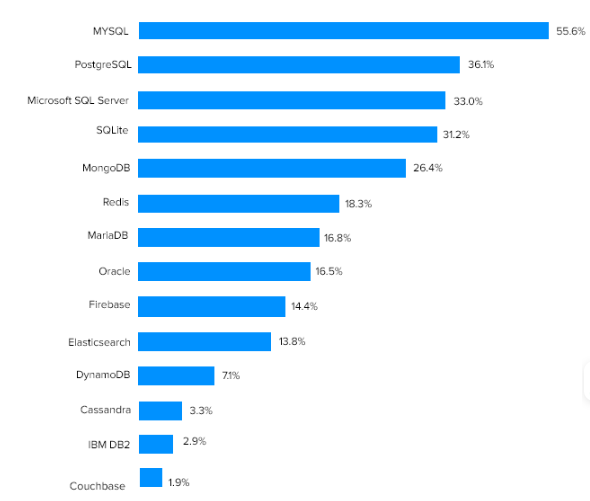
\includegraphics[scale=0.6]{images/top14_database.png}
\caption{14 legnépszerűbb adatbázis\cite{databases}}.
\label{fig:Adatbázisok}
\end{figure}
\newpage

\Section{Front-end}

A frontend a szoftver megjelenítési rétege. A weboldalnak azon rétege, amit a felhasználó is lát, és interakcióba tud vele lépni. Legfontosabb része a HTML (Hypertext Markup Language), ez adja meg a weboldal kinézetének a vázát, és hozzá csatlakozik a CSS (Cas-cading Style Sheets), ami segítségével egyedi megjelenést biztosíthatunk a weboldalunknak. Több fajta keretrendszer létezik Front-end fejlesztésre, mint például:

\begin{itemize}
\item React,
\item Angular,
\item Vue.js.
\end{itemize}


\subsection{Angular}

Az Angular egy TypeScript-alapú, nyílt forráskódú webalkamazás-keretrendszer. 2016-ban jelent meg az első verzió.

Egyben tartalmazza a TypeScript osztályt HTML-sablont stílusokkal. A HTML sablon lehetővé teszi dinamikus értékek beszúrását, mint például szöveg, tartalmaz komponenseket, amelyek NgModulokba vannak rendezve. Minden alkalmazásnak van egy úgynevezett gyökérmodulja, aminek a neve általában az AppModule, amely a bootstrap mechanizmust biztosítja, amely elindítja az alkalmazást. Ngmodulok is importálhatnak más Ngmodulokat, például az útválasztó szolgáltatás használatához a Router NgModul-t.  Minden Angular alkalmazásnak van egy gyökérkomponense, ami összekapcsolja a komponens hierarchiát. Mindegyik komponenshez tartozik egy HTML-sablon, amely segítségével megjeleníthető a tartalom. Tartalmaz egy services osztályt is. Ezt akkor használjuk, ha van olyan adat vagy logika, amelyek nem kapcsolódnak, de meg szeretnénk osztani a komponensek között\cite{Angular}.

\Section{Fejlesztői környezetek és fejlesztéshez használt p-rogramok}

\subsection{Intelij IDEA}

Az InteliJ IDEA Egy integrált fejlesztői környezet amit a JetBrains fejlesztett ki. Ebben az IDEA-ban Java, Kotlin, Groovy és más JVM alapú nyelveken írt szoftvereket lehet fejleszteni. Az integrált fejlesztői környezet (IDE)  egy olyan  szoftveralkamazás, amely átfogó lehetőségeket biztosít a számítógép programozóknak a szofverfejlesztéshez . Az IDE általában legalább egy forráskódszerkesztőből, építési autómatizálási eszközökből, és egy hibakeresőből áll. Egyes IDE-k, például a NetBeans és az Eclipse tartalmazzák a szükséges fordított, értelmezőt vagy mindkettőt; mások, például a SharpDevelop és a Lazuras nem\cite{Intelij}\cite{Intelij2}.

\begin{figure}[h]
\centering
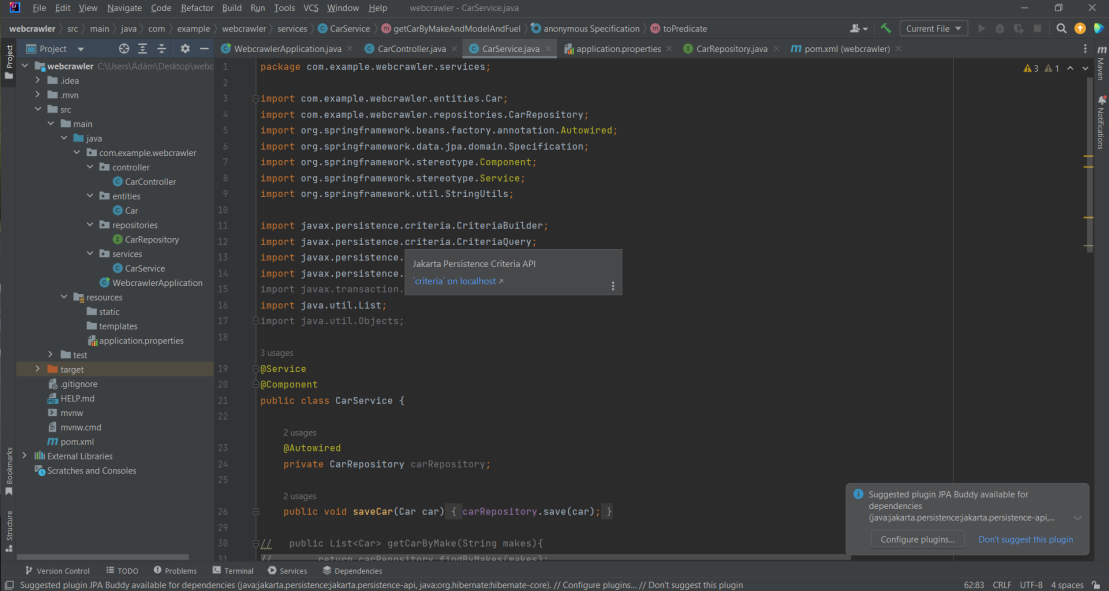
\includegraphics[scale=1]{images/Intelij.png}
\caption{Intelij IDEA.}
\label{fig:Intelij}
\end{figure}

\subsection{Visual Studio Code}

VS Code egy forráskód szerkesztő, amit a Microsoft fejlesztett ki 2015-ben\cite{VSCode}. Windows, Linux és MacOS operációs rendszereken érhető el. Nagyon sok programozási nyelvel lehet használni, mint például:

\begin{itemize}
\item JavaScipt,
\item Go,
\item Node.js,
\item C++,
\item Phyton.
\end{itemize}

Rengeteg kiegészítővel lehet bővíteni a fejlesztő környezetet, ami könnyebbé és átláthatóbbá teszi a fejlesztést, ezért esett a választásom erre a környezetre a frontend fejlesztéséhez.

\begin{figure}[h]
\centering
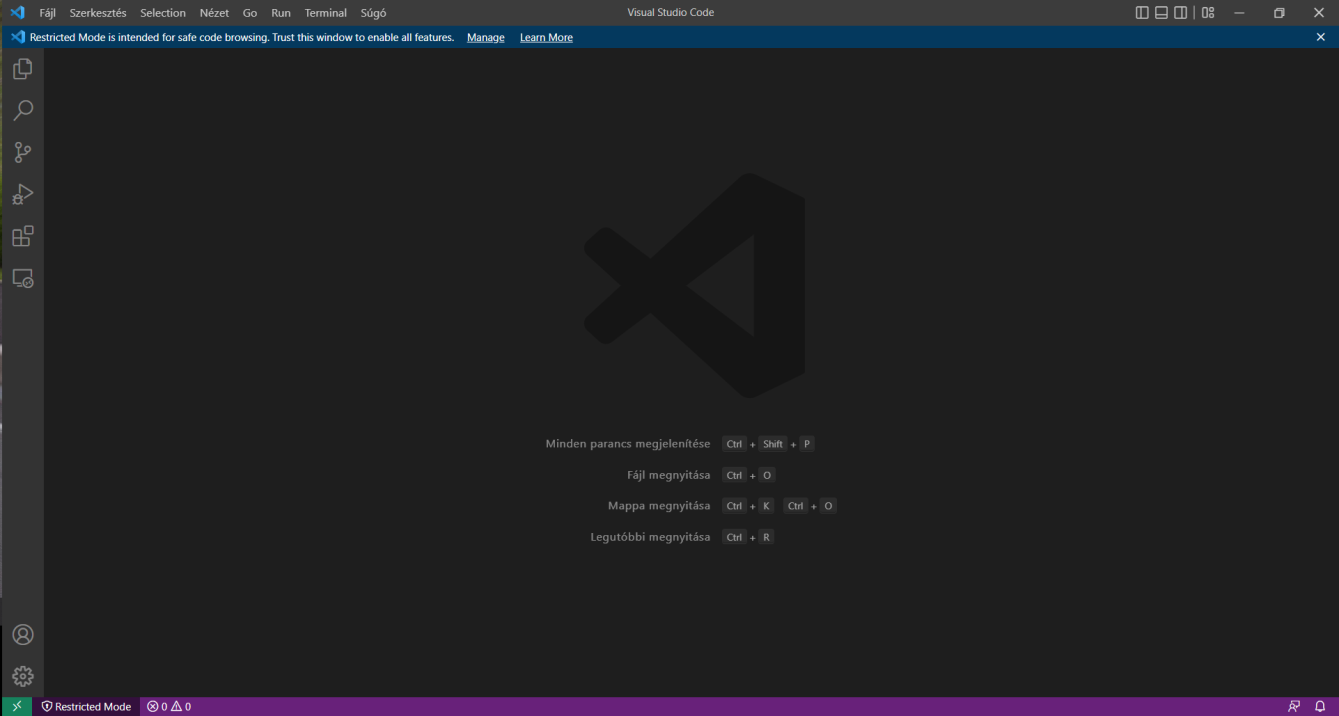
\includegraphics[scale=0.6]{images/VSCode.png}
\caption{Visual Studio Code.}
\label{fig:VSCode}
\end{figure}
\newpage

\subsection{Postman}

A Postman \cite{Postman} API-k létrehozására és használatára, tesztelésére létrehozott platform. Használatával egyszerűbben és gyorsabban hozhatunk létre jobb minőségű API-kat. Rengetek eszközkészletet tartalmaz, amely tovább gyorsítja az API létrehozását a  tervezéstől egyenesen a tesztelésig. Ilyen eszközök a következők:

\begin{itemize}
\item API kliens: Lehetővé teszi API-k tesztelését, hibakeresését, és van lehetőség HTTP, REST, SOAP és GraphQL kéréseket is indítani.
\item API tervezés: OpenAPI, RAML, GraphQL vagy SOAP formátumban tervezhetjük meg az API-kat. A Postman Schema szerkesztője megkönnyíti a különböző méretű fájlokkal való munkát.
\item API dokumentáció: Postman automatikusan géppel olvasható dokumentációt hoz létre, amit OpenAPI-fájlokon keresztül dokumentál. Tartalmazza a kérések részleteit mintakódokkal.
\item API tesztelés: Lehetőség van használni funkcionális teszteket, integrációs teszteket, regressziós teszteket. A Postman egy Node.js alapú futtatókörnyezet, ami támogatja gyakori mintákat és  könyvtárakat, ami segíti a gyors tesztkészítést.
\item Monitorozás: Naprakészek lehetünk az API állapotával és teljesítményével kapcsolatban. A monito-
rok a Postman felhőjében vannak tárolva, és ennek köszönhetően gyorsan beállíthatjuk őket.
\item Mock szerverek: Más néven „Áll szerverek” aminek segítségével láthatjuk hogyan fog futni az API-nk mielőtt kihelyeznénk az éles környezetbe. A Postman felhő üzemelteti, és így bárhonnan elérhetőek.
\end{itemize}

\begin{figure}[h]
\centering
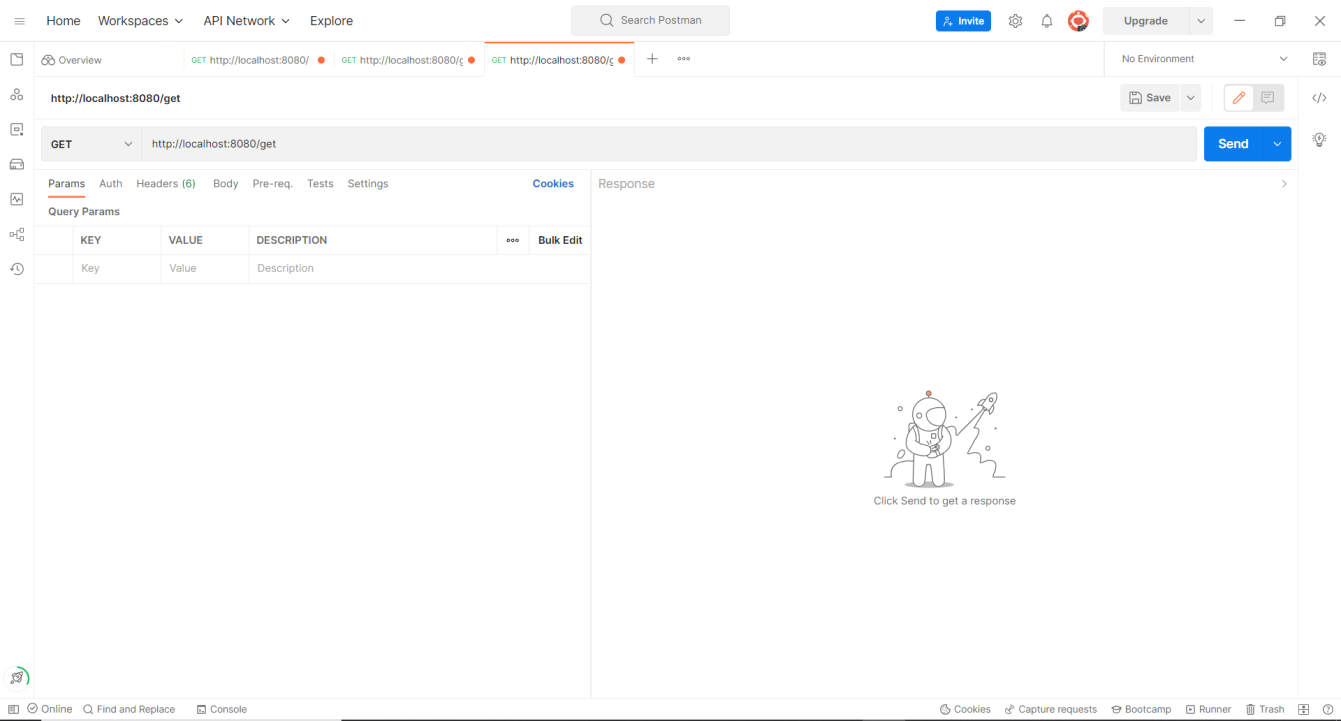
\includegraphics[scale=0.8]{images/Postman.png}
\caption{Postman.}
\label{fig:Postman}
\end{figure}
\newpage

\subsection{PgAdmin}

A PgAdmin\cite{PgAdmin} egy grafikus felhasználói felület a PostgreSQL kezelésére, ami a lehető legjobb megoldás lehet, mert nagyon hatékonyan lehet velük dolgozni. Legújabb verziója a PgAdmin 4, jQuery, JavaScript és Python kombinációjával készült. Előnyei, hogy:

\begin{itemize}
\item kompatibilis Windows, Linux és MacOS operációs rendszerekkel is,
\item bárhova telepíthető ahol PostgreSQL-t használunk,
\item van olyan lekérdező eszköze, amivel gyorsabb az adatbevitel és a hibakezelés.
\end{itemize}

Rengeteg dokumentáció megtalálható hozzá amivel könnyedén el lehet kezdeni a használatát.

\begin{figure}[h]
\centering
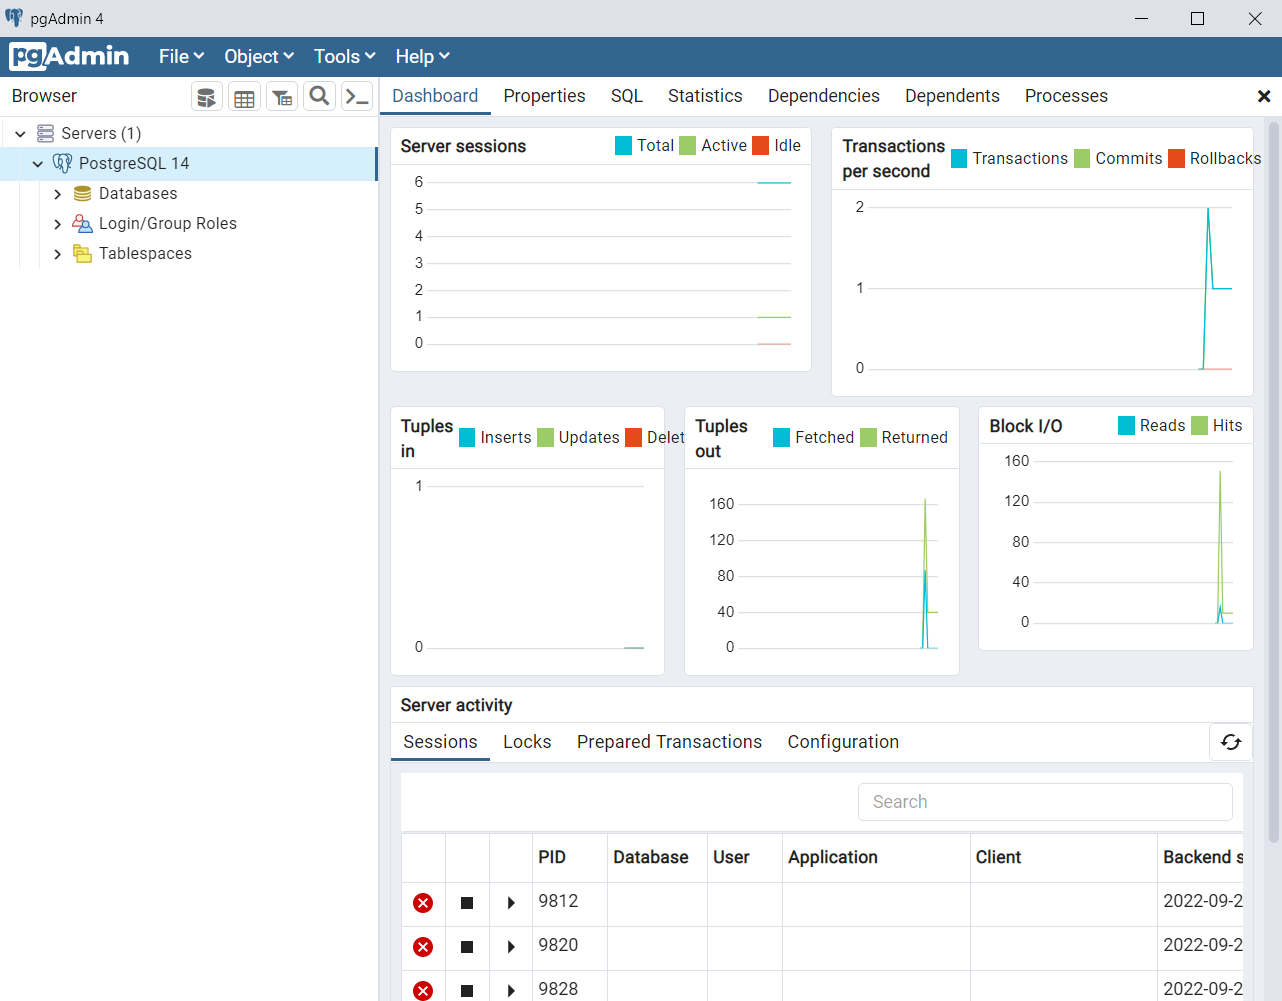
\includegraphics[scale=0.3]{images/PgAdmin.png}
\caption{PgAdmin 4.}
\label{fig:PgAdmin 4}
\end{figure}
\newpage

